La chitarra ha una lunga tradizione che affonda le sue radici addirittura al tempo degli arabi. I primi esemplari risalgono al tredicesimo secolo. Inizialmente dotata di quattro corde, si è accresciuta nel Rinascimento di un'altra corda, arrivando poi nel periodo Barocco all'attuale numero di sei.\\
\newline
La chiatarra è composta da due parti principali:
\begin{itemize}
	\item il manico, su cui si trova la tastiera e che termina con la paletta la quale ospita le meccaniche per l'accordatura;
	\item la cassa di risonanza o tavola armonica con una cavità centrale, che serve ad amplificare il suono prodotto dalle corde.
\end{itemize}

\begin{figure}[H]
	\centering
	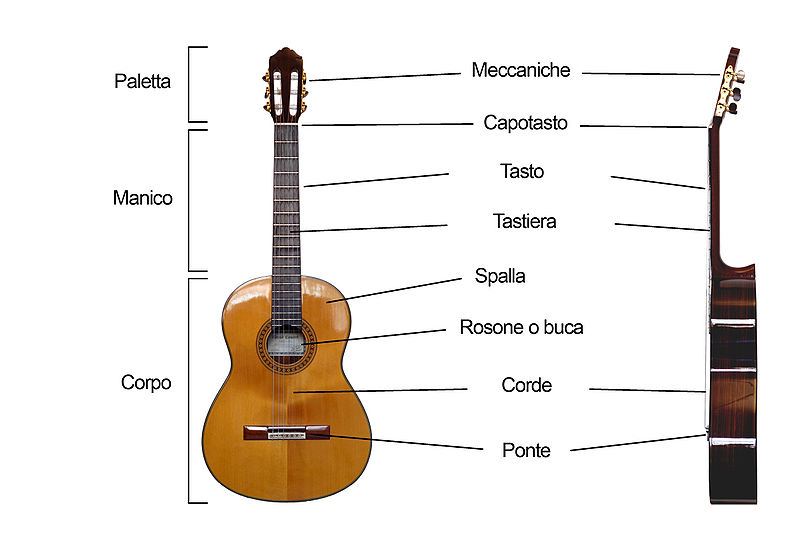
\includegraphics[scale=0.50]{./images/img14.jpg}
\end{figure}

\subsection{Corde}
Le corde delle chitarre moderne sono sei e sono ordinate dall'alto verso il basso nel seguente modo:
\begin{itemize}
	\item la prima corda corrisponde alla nota Mi cantino (e);
	\item la seconda corrisponde alla nota Si (B);
	\item la terza corrisponde alla nota Sol (G);
	\item la quarta corrisponde alla nota Re (D);
	\item la quinta corrisponde alla nota La (A);
	\item la sesta corrisponde alla nota Mi basso (E).
\end{itemize}
L'ultima corda dell'elenco è quella più spessa, mentre la prima è la più sottile.
\subsection{Tasti}
Sul manico della chitarra c’è la tastiera. Si chiama tastiera proprio perchè ci sono i tasti. Quest'ultimi sono delimitati da delle barrette di metallo e ognuno di essi corrisponde a una nota. Dunque, se abbiamo una chitarra a 19 tasti, possiamo fare 19 note diverse per ogni corda.\\
La distanza tra due tasti della stessa corda prende il nome di \textbf{semitono}. Ad esempio, se premiamo la sesta corda in corrispondenza del La, poi premendo la corda al tasto adiacente più vicino alla cassa di risonanza (un semitono più alto) ascolteremo un La\#.\\
Se non premiamo nessun tasto la corda si dice che è suonata a vuoto. Le sei corde suonate a vuoto devono emettere dei suoni ben precisi: la chitarra deve essere quindi accordata. L'accordatura classica delle sei corde, ovvero la nota che devono suonare le corde a vuoto (dal basso all'alto), è la seguente: Mi, La, Re, Sol, Si, Mi.\\
Conoscendo il suono prodotto dalle sei corde suonate a vuoto e sapendo che ogni nota suonata ad un tasto dista di un semitono dalla nota suonata al tasto adiacente possiamo mappare tutta la tastiera della chitarra.
\begin{figure}[H]
	\centering
	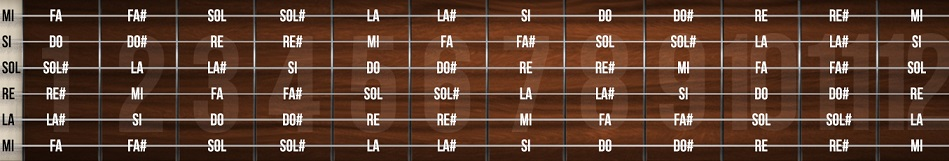
\includegraphics[scale=0.60]{./images/img13.jpg}
\end{figure}

\subsection{Tab}
La \textit{tab} è una rappresentazione delle corde della chitarra. Una tablatura è solitamente scritta usando sei linee orizzontali, ognuna corrispondente a una corda.\\
Al contrario dei normali spartiti, su una tablatura non ci sono le note da suonare ma si trovano le indicazioni su dove mettere le dita. I numeri sulle linee corrispondono ai tasti della tastiera. Ad esempio, un "1" sulla prima corda, indica di suonare il Mi cantino tenendo premuto il primo tasto.
Se il numero è superiore a zero, bisogna premere il tasto corrispondente quando si suonerà quella corda. Se troviamo uno \textbf{zero} allora si suona la corda a vuoto, senza premere alcun tasto.
\begin{figure}[H]
	\centering
	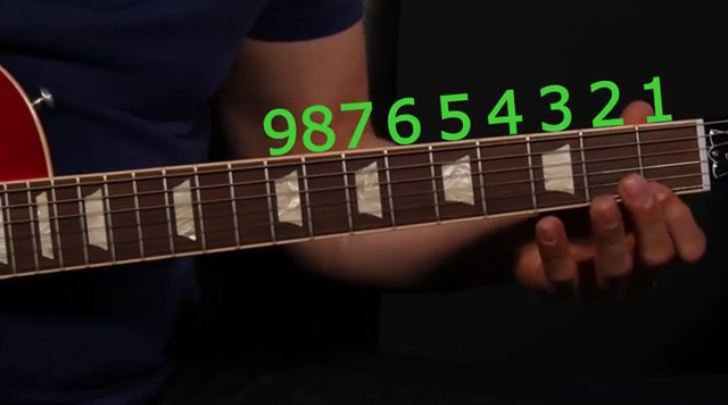
\includegraphics[scale=0.50]{./images/img15.png}
\end{figure}

Spesso leggendo una tablatura si trovano dei numeri che sono allineati verticalmente. In questo caso si premono più tasti contemporaneamente. Le tab vanno lette come libri cioè da sinistra a destra.
\begin{figure}[H]
	\centering
	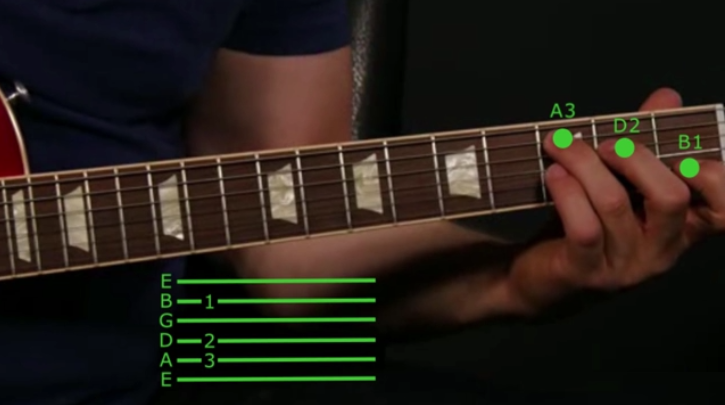
\includegraphics[scale=0.50]{./images/img16.png}
\end{figure}